\documentclass[border=2pt]{standalone}
\usepackage{tikz}
\usepackage{pgfplots}
\pgfplotsset{compat=1.18}
\usepgfplotslibrary{fillbetween}

% Brand colors
\definecolor{Garnet}{rgb}{0.451, 0.0, 0.039}
\definecolor{Atlantic}{rgb}{0.275, 0.416, 0.624}
\definecolor{Congaree}{rgb}{0.122, 0.255, 0.302}
\definecolor{Horseshoe}{rgb}{0.396, 0.471, 0.043}
\definecolor{Black90}{rgb}{0.212, 0.212, 0.212}
\definecolor{Black50}{rgb}{0.635, 0.635, 0.635}

\begin{document}
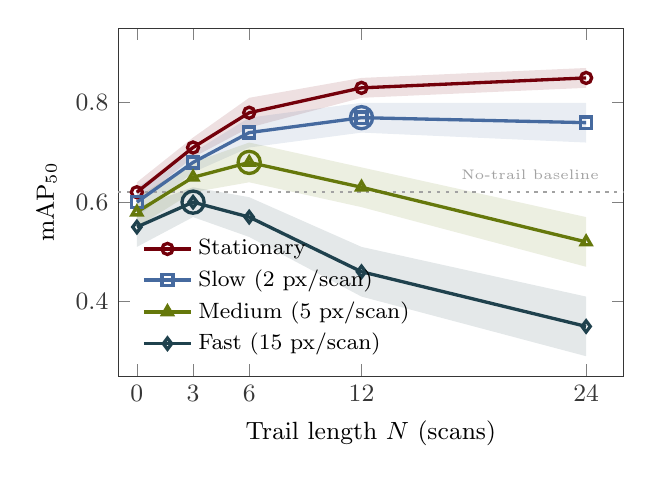
\begin{tikzpicture}
\begin{axis}[
  width=8cm,
  height=6cm,
  xmin=-1, xmax=26,
  ymin=0.25, ymax=0.95,
  xlabel={Trail length $N$ (scans)},
  ylabel={mAP$_{50}$},
  xlabel style={font=\small},
  ylabel style={font=\small},
  xtick={0,3,6,12,24},
  axis line style={Black90},
  tick label style={font=\small, color=Black90},
  legend style={
    at={(0.03,0.03)},
    anchor=south west,
    draw=none,
    fill=none,
    font=\footnotesize,
    cells={anchor=west}
  },
  rounded corners=0pt,
  every axis plot/.append style={line width=1.2pt}
]

% No-trail baseline reference
\addplot[Black50, dotted, line width=0.8pt, forget plot]
  coordinates {(-1,0.62) (26,0.62)};
\node[font=\tiny, color=Black50, anchor=south east] at (axis cs:25.2,0.625) {No-trail baseline};

% Stationary
\addplot[color=Garnet, mark=o, mark size=2pt]
  coordinates {(0,0.62) (3,0.71) (6,0.78) (12,0.83) (24,0.85)};
\addlegendentry{Stationary}
\addplot[name path=stat_upper, draw=none, forget plot]
  coordinates {(0,0.64) (3,0.73) (6,0.81) (12,0.85) (24,0.87)};
\addplot[name path=stat_lower, draw=none, forget plot]
  coordinates {(0,0.60) (3,0.69) (6,0.75) (12,0.81) (24,0.83)};
\addplot[Garnet, opacity=0.12, forget plot] fill between[of=stat_upper and stat_lower];

% Slow
\addplot[color=Atlantic, mark=square, mark size=2pt]
  coordinates {(0,0.60) (3,0.68) (6,0.74) (12,0.77) (24,0.76)};
\addlegendentry{Slow (2 px/scan)}
\addplot[name path=slow_upper, draw=none, forget plot]
  coordinates {(0,0.63) (3,0.70) (6,0.77) (12,0.80) (24,0.80)};
\addplot[name path=slow_lower, draw=none, forget plot]
  coordinates {(0,0.57) (3,0.66) (6,0.71) (12,0.74) (24,0.72)};
\addplot[Atlantic, opacity=0.12, forget plot] fill between[of=slow_upper and slow_lower];

% Medium
\addplot[color=Horseshoe, mark=triangle, mark size=2pt]
  coordinates {(0,0.58) (3,0.65) (6,0.68) (12,0.63) (24,0.52)};
\addlegendentry{Medium (5 px/scan)}
\addplot[name path=med_upper, draw=none, forget plot]
  coordinates {(0,0.61) (3,0.68) (6,0.72) (12,0.67) (24,0.57)};
\addplot[name path=med_lower, draw=none, forget plot]
  coordinates {(0,0.55) (3,0.62) (6,0.64) (12,0.59) (24,0.47)};
\addplot[Horseshoe, opacity=0.12, forget plot] fill between[of=med_upper and med_lower];

% Fast
\addplot[color=Congaree, mark=diamond, mark size=2pt]
  coordinates {(0,0.55) (3,0.60) (6,0.57) (12,0.46) (24,0.35)};
\addlegendentry{Fast (15 px/scan)}
\addplot[name path=fast_upper, draw=none, forget plot]
  coordinates {(0,0.59) (3,0.63) (6,0.61) (12,0.51) (24,0.41)};
\addplot[name path=fast_lower, draw=none, forget plot]
  coordinates {(0,0.51) (3,0.57) (6,0.53) (12,0.41) (24,0.29)};
\addplot[Congaree, opacity=0.12, forget plot] fill between[of=fast_upper and fast_lower];

% Optimal N markers (open circles)
\addplot[Atlantic, mark=o, mark size=4pt, only marks, line width=1.2pt, forget plot]
  coordinates {(12,0.77)};
\addplot[Horseshoe, mark=o, mark size=4pt, only marks, line width=1.2pt, forget plot]
  coordinates {(6,0.68)};
\addplot[Congaree, mark=o, mark size=4pt, only marks, line width=1.2pt, forget plot]
  coordinates {(3,0.60)};

\end{axis}
\end{tikzpicture}
\end{document}
